% !TEX TS-program = pdflatex
% !TEX encoding = UTF-8 Unicode

% Example of the Memoir class, an alternative to the default LaTeX classes such as article and book, with many added features built into the class itself.

%\documentclass[12pt,a4paper]{memoir} % for a long document
\documentclass[11pt,a4paper,article]{memoir} % for a short document
\raggedbottom
\raggedright

\usepackage[utf8]{inputenc} % set input encoding to utf8
\usepackage{graphicx}
\usepackage{amsmath}
\usepackage{caption}
\usepackage{float}
\usepackage{parskip}
\usepackage{mathpazo}
\usepackage{lscape}
\usepackage{mdwlist}

\setlength{\parskip}{\baselineskip}%
\setlength{\parindent}{0pt}%

%%% PAGE DIMENSIONS
% Set up the paper to be as close as possible to both A4 & letter:
\settypeblocksize{*}{13cm}{1.8} 
\setulmargins{*}{*}{1} % 50pt upper margins
\setlrmargins{*}{*}{1}% golden ratio again for left/right margins
\setheaderspaces{*}{*}{1.618}
\checkandfixthelayout 
% This is from memman.pdf

%%% ToC (table of contents) APPEARANCE
\maxtocdepth{subsection} % include subsections
\renewcommand*{\cftappendixname}{Appendix\space}

%%% HEADERS & FOOTERS
\pagestyle{plain} % try also: empty , plain , headings , ruled , Ruled , companion

%%% CHAPTERS
\chapterstyle{section} % try also: default , section , hangnum , companion , article, demo

%%% SECTIONS
\hangsecnum % hang the section numbers into the margin to match \chapterstyle{hangnum}
\maxsecnumdepth{subsection} % number subsections

\makeatletter
\renewcommand\tableofcontents{%
\null\hfill\textbf{\huge\contentsname}\hfill\null\par
  \vspace{14pt}
  \@mkboth{\MakeUppercase\contentsname}{\MakeUppercase\contentsname}%
  \@starttoc{toc}%
}

\renewcommand\contentsname{Table of Contents}
\makeatother
\renewcommand{\baselinestretch}{1.5} 
\graphicspath{{./images/}}


%% MY COMMANDS


%% RUBRIC %%%%%%%%%%%%%%%%%%%%%%%%
% Style pointers
% > Write in the past tense
% > Passive
% > 'Each paragraph should contain a complete thought or argument'

% RUBRIC
% ---------------------------------------------------------------------------------
% Communication
% 	> Abstract
% 	> Clear statement of aims/objectives
% 	> Overall quality of report:
%		- Structure
%		- Appearance
%		- Use of English
%		- Grammar
%		- Typographical errors
%		- Nomenclature
%		- Symbols
%		- Acronyms
%		- References
% 	> Introduction to process/method
% 	> Background of industry/company context
% 	> Presentation and discussion of work and results
% 	> Conclusions and recommendations for further work
% 	> Quality of diagrams, tables
% 	> Sufficient references
% \/* "The report is well organised and well presented
% with excellent use of figures, tables and
% references. There are no spelling or grammatical
% errors. Complex information is communicated in a
% clear and logical manner." */
% \/*The purpose of the Industrial Critique report is to show that you can take an overview of a
% process, methodology or design exercise that you have personally had direct experience of, or
% been involved with, during your placement.*/
% STRUCTURE
% > Introduction
%		What DCA do, who their competitors are
%		What statistics is
%			Generic process overview
%				1. Design 2. Execute 3. Analyze 4. Present
%		Relevance of statistics to DCA
%		Outline of report structure
% > Overview of current methods
%		How DCA currently uses statistics
%			Process diagram
%			Analysis, experiment design, presentation/visualization
%			Evaluation
%		How DCA's competitors currently use statistics
%			Summary
%			Evaluation and comparison
% > Proposed alternatives
%		What methods DCA could use instead
%			Concepts
%				Analysis - Linear models (simple, multivariable, basis expansion, analysis of variance)
%				Experiment design - Blocking, factorial designs, and Taguchi
%				Data visualization - scatter and box plots, histograms
%			Implementation
%				Matlab, R, Minitab, Excel, Python
% > Conclusion

% Content
%	> Understanding of appropriate theory
%	> Understanding of process/method described
%	> Understanding of alternatives discussed
%	> Evaluation of alternatives discussed
%	> Critical discussion of work
%\/* The report is authoritative and the proposals/options
% described are suitable for implementation. An
% innovative approach is evident and there is a
% thorough awareness of the issues around
% implementation and of the economic feasibility of the
% proposals made. */
% B) How outcomes and results were checked and/or verified in DCA
% C) What went well and what did not go so well in the way statistics is done at DCA
% D) ALternative processes methods which could have been used toghther with the procs and cons of each of each of these
% E) Recommendations for improvements that could be made to the process used, giving details of the implications of these
% The focus of this critique is not on the detail of what you did or achieved but on your wider and
% deeper understanding of how the work was carried out, why it was carried out in the way it was,
% and on the alternative approaches that could have been taken. Technical detail is not a
% fundamental requirement of the critique (though should be included at an appropriate level) – it is
% the evaluation of the process/methodology that is important.

% Consider both operational and financial implications of the alternatives recommended.

% The ICR requires that you detail a critique of a process, methodology or design exercise. You are
% expected to evaluate the pros and cons of alternative approaches which may not be is use in your
% placement company and will therefore require you to carry out some research into what your
% company does and what is done elsewhere. The report must also make some recommendations,
% which may also propose further evaluation or work to implement and changes you are proposing.
% You may also need to support your conclusions and recommendations with some quantitative
% assessments of time, cost, efficiency improvements etc.

%%%%%%%%%%%%%%%%%%%%%%%%%%%%%%





%%% TITLE PAGE
\newlength\drop
\makeatletter
\newcommand*\titleM{\begingroup% Misericords, T&H p 153
\setlength\drop{0.1\textheight}
\centering
\vspace*{\drop}
{\Huge\bfseries Statistics \vspace{14pt} for \vspace{14pt}  Product Development}\\ 
\vspace{1in}
{Jerome Wynne}\\[\baselineskip]
{\scshape University of Bristol}\par
\vspace{0.61in}

%%% ABSTRACT %%
% – Set the scene (background)
% – State why the topic of your ICR is important (within the
% context of the background)
% – State why/how what was done is different or unique (or
% why it was carried out)
% – Briefly summarise results, conclusions and
% recommendations
{\bfseries Abstract}\\[\baselineskip]
{Analyzing a product's performance during development is essential to making informed design decisions, yet many engineers are uncomfortable using statistics. This shouldn't be the case: statistical tools can be invaluable for recognizing patterns in experimental data, and therefore offer a means of improving the quality and consistency of design decisions. Here, DCA's current use of statistics is evaluated relative to modern statistical practice. Experiment design, analysis, and presentation tools are suggested that would enhance DCA's testing process. These tools are evaluated against the realities of DCA's work by considering how they might be implemented in DCA's experimental procedures.}
\vfill

{\scshape \@date}\par
\endgroup}
\makeatother

% MULTILINE COMMENTS
\long\def\/*#1*/{}

%% START OF DOCUMENT
\begin{document}

\begin{titlingpage}
\titleM
\end{titlingpage}

\tableofcontents* % the asterisk means that the contents itself isn't put into the ToC
\firmlists

% List of tables/figures
\newpage
\listoftables
\listoffigures

% Notation
\newpage
\chapter*{Notation \& Glossary}
\begin{tabular} {p{2.7cm}p{10cm}}
\textbf{Attribute} & A measurable property of a \textit{unit}. \\[0.5cm]
\textbf{Block} & A set of \textit{units} thought to share some common \textit{attribute} that influences their \textit{response}. \\[0.5cm]
\textbf{Event} & A set of \textit{outcomes}.\\[0.5cm]
\textbf{Experiment$^{1}$} & The controlled collection of data. \\[0.5cm]
\textbf{Experiment$^{2}$} & Physically realizing an outcome of the system under study. \\[0.5cm]
\textbf{Factors} & \textit{Treatments} that are discrete. For example, lubricated/unlubricated.\\[0.5cm]
\textbf{Outcome} & A possible result of a \textit{trial}. \\[0.5cm]
\textbf{Probability} & A method for quantifying uncertainty, or a value representing the uncertainty of an event. \\[0.5cm]
\textbf{Response} & The measured performance of a \textit{unit}. \\[0.5cm]
\textbf{Treatment} & A modification applied to a \textit{unit}.\\[0.5cm]
\textbf{Unit} & A single test specimen - in the context of product testing, this is likely to be a prototype build of the product.
\end{tabular}

\newpage
\chapter*{\large Acknowledgements}
\vspace*{-\baselineskip}
Beyonc\'{e}, J.D.Sallinger, and Santa Claus. \\
This report would not have been possible without the encouragement of Paul Harper and technical supervision of Sophie Sladen. More broadly, I am grateful to DCA Design International for providing me a place to work on these ideas and develop professionally. Thank you to DCA's engineers - especially Will Marsh, Matthew Jones,   and Matthew Edwards - for setting the bar so high and for helping me to improve as an engineer.
\chapter*{\large Declaration}
\vspace*{-\baselineskip}
I confirm that the work presented here is wholly my own and has been generated as a result of my own thought and study. Where I have consulted the work of others it is mentioned, and where my work was part of a group effort my contribution is made clear. Where the work of another is quoted, the source is given.



%% INTRODUCTION %%
\newpage
\chapter{Introduction}
% A) Why statistics was used in DCA
DCA Design International is a 150-person product design consultancy based in Warwick. Their work is oriented towards the mechanical design of medical and consumer products. Much of what they develop is hand-held items such as insulin injector pens or deoderant cans. DCA's competitors are [DCA's COMPETITORS AND THEIR CAPABILITIES].
\par
DCA employs about sixty mechanical engineers. Each of them are general-purpose technical consultants and experts in a particular engineering subdiscipline. DCA's substantial investment in engineering distinguishes it from other product design consultancies, many of which do not have the facilities to handle a product's technical development [REFERENCE]. This investment is manifest in both the its engineering workforce and its ownership of four test labs. The experiments run in these labs and the data they produce is the focus of this report. 
\par
This equipment is regularly used by DCA's engineers to generate experimental data. The way in which this data is collected, analyzed, and presented is the focus of this report: data-oriented activities constitute the scientific discipline of statistics. Statistical methods allow resources and information to be used efficiently, in both a mathematical sense and a practical one.
\par
Section X1 explains the company's current investigatory framework and how statistics is currently applied within it. In Section X2 the company's approach is compared to modern statistical methods, in the process of which these alternative methods are detailed and evaluated. Tools (i.e. software and tangibles) for implementing statistical methods are also discussed in the context of DCA's needs. The report concludes with an evaluation of how actionable the suggested methods are, and responds to hypothetical criticisms of the relevance of statistics in a product design consultancy.

\newpage



%% DCA'S USE OF STATISTICS IN LAB INVESTIGATIONS %%
\chapter {Overview of DCA's Use of Statistics}
This section contextualizes DCA's uses of statistics and explains what methods are currently being applied by its engineers. Each method is critiqued according to its use case.
\section{The Structure of a Lab Investigation in DCA}
% What does a testing sequence look like?
It's convenient to split the statistical methods that DCA apply into two factions: those brought to bear in lab investigations, and those used in other engineering activities, in particular tolerance analysis and predictive modelling for product interfaces.
\par
A lab investigation in DCA consists of a series of experiments to understand the behaviour of a product or process. It begins with the required knowledge being identified. Experiments will then be designed, executed, and analyzed until the knowledge is acquired or is deemed no longer relevant. This process is depicted in Figure \ref{fig:investigation_diagram}.
\begin{figure}[h!]
\centering
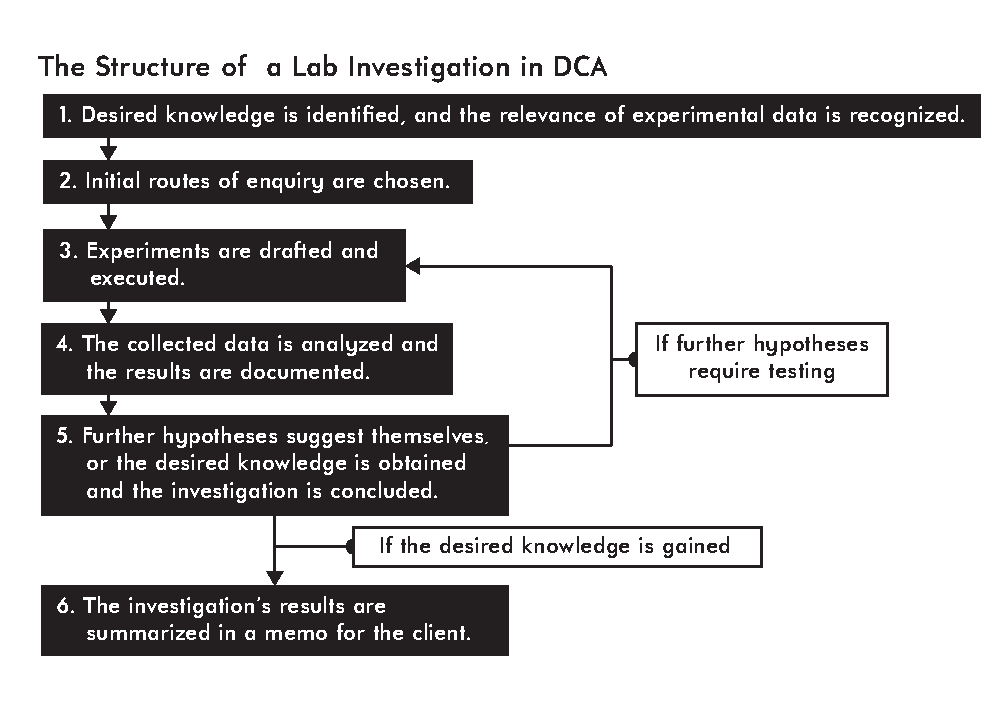
\includegraphics[width=1.2\textwidth]{Lab_Investigation_Diagram.pdf}
\caption{Investigation diagram.}
\label{fig:investigation_diagram}
\end{figure}
% What departments in DCA test their products?
All aspects of an investigation - from experiment design through to presenting the results to a client - are handled by engineers assigned to the relevant project. Typically an investigation focuses on a particular product parameter, such as the volume of fluid dispensed by an injector, or the propensity of a inhaler to fail upon being dropped. 
\par
As can be seen in Figure \ref{fig:labwork_breakdown}, most lab work is conducted by engineers on medical projects.
Occasionally engineers working on fast-moving consumer goods (such as toothbrushes or lotion bottles) will run one-off tests to compare design variations or verify performance relative to some baseline. In general however, the timeframes and functional requirements of such products limit the relevance of extensive experimental investigations to them: medical products on the other hand, see a good deal of the test lab.
\par
% When do they test them and why?
As can be seen in Figure \ref{fig:time_of_tests}, most experiments are run in the late stages of the design process. This is when resolving minor performance issues becomes a worthwhile pursuit, exploration for future product variants become a possibility, and rehearsal for fast-approaching regulatory tests becomes essential.
\begin{figure}
\label{fig:time_of_tests}
\end{figure}
\par
% How do they test them?
DCA's engineers have access to axial and torsional testing machines, environment chambers, coordinate measuring machines, mass balances, and high-speed cameras, among other engineering instruments. Investigations commonly revolve around a particular experimental set-up, however ancillary experiments are often designed to provide supplementary information. With this in mind, it is worth noting that this report attempts to be data-agnostic in its recommendations of analytical techniques.
\par
The other engineering activities that DCA's engineers apply statistics to are tolerance analysis and, increasingly, predictive user interfaces. Before talking about this work however, DCA's use of statistics in its lab investigations will first be summarized and critiqued.

%%
\section{Experiment Design}
Experimental design and analysis can be used to make products that perform better, are more reliable, less risky to develop, and have a uniquely justifiable development process. It is expertise that would elevate DCA's capacity as a technical consultancy.
\par
Design of Experiments refers to both experiment designs and a broader philosophy of systematic experimentation. An experiment design is a particular structure of experiment, such as comparing the effects of two factors each at two levels. Good experimental design produces data that is relevant to the experiment's objective and is logically unambiguous.
\par
Robust experiments are designed with three features in mind:
\begin{description}
\item[Replication]{Testing a particular combination of factor levels with more than one unit. It allows us to estimate experimental error and to obtain a more precise estimate of a particular factor's influence.}
\item[Randomization]{Randomly determining the allocation of treatments to units and the sequence in which units are tested averages out the effects of nuisance variables, and validifies the assumption that units are randomly drawn from a particular distribution.}
\item[Blocking]{Accounting for possibly important differences between units when assigning treatments. A block is a set of similar units.}
\end{description}
These principles constitute the makings of any well-designed experiment, and they are evident in DCA's labwork: units are blocked according to factors such as component batches and time of assembly, testing and assembly sequences are randomized, and engineers fret about their sample sizes. Engineers in DCA iterate on test fixtures until they are satisfied that what's being observed is representative of the system under study - their scepticism is commendable.
\par
The greatest strength of DCA's experiments is their procedural simplicity. 
\par
This being said, DCA neglect pre-experimental planning and lack the expertise to apply more sophisticated experiment designs when they are needed. Further, it is uncomfortable handling resource-limited investigations, and has an inconsistent approach to determining important design factors in large solution spaces, resulting in mired investigations.
\par
These principles are discussed implicitly every time an engineer in DCA frets about choice of component batch, sequence of testing, and the sufficiency of a sample size. 
\par
DCA's application of experiment design at present is evaluated against a traditional experimental procedure in Table \ref{table:exp_procedure}.
TABLE
\bgroup
\def\arraystretch{1.5}
\begin{landscape}
\begin{table}
\begin{tabular}{|p{8cm}|p{5cm}|p{5cm}|p{5cm}|}
\hline
\multicolumn{1}{|c|}{\bfseries Experimental Step}		&	\multicolumn{1}{c|}{\bfseries DCA's Implementation}	& \multicolumn{2}{c|}{\bfseries Evaluation}	\\
\hline
1. Recognition and statement of the problem. 			&		Dummy text.		&		 Some text more text more text more text			& 	 Some moooore text again \\
						 			&					&		 Another text		& 	 txt 2 \\
\hline
2. Choice of factors, levels, and ranges.		&		Dummy text.		&		Dummy text 	& 	csdfsd \\
\hline
3. Selection of the response variable.			&		Dummy text.		&		Dummy text  & 	csdfsd \\
\hline
4. Choice of experimental design.			&		Dummy text.		&		Dummy text 	& 	csdfsd  \\
\hline
5. Performing the experiment.				&		Dummy text.		&		Dummy text 	& 	csdfsd  \\
\hline
6. Statistical analysis of the data.			&		Dummy text.		&		Dummy text 	& 	csdfsd  \\
\hline
7. Conclusions and recommendations.			&		Dummy text.		&		Dummy text 	& 	csdfsd  \\
\hline
\end{tabular}
\end{table}
\end{landscape}
\egroup
\par
Several experiment designs dominate in the company: these are enumerated, explained, and critiqued in Table 2.
TABLE
\begin{description}
\item[Best-guess approach]{Factor levels for a test are chosen according to the results of a previous test. One or two factors at a time are varied in this way. \\ - No guarantee of optimal solution \\ - Can continue indefinitely.}
\item[One-factor-at-a-time]{A baseline set of factor levels are chosen, then each factor is varied across its range while all other factors are held at this baseline.\\ - Does not consider interactions \\ - Resource inefficient}
\item[Simple comparative]{}
\item[Factorial]{All possible combinations of factor levels are tested.}
\end{description}


DCA certainly follow this structure, however it is implemented haphazardly across the company. For example, there is no formal guidance for steps 1-4, 6, or 7. This could result in several problems:
\begin{itemize}
\item Overlooking important properties of the problem at hand that may become apparent only when running an experiment, or that may not become apparent but would seriously influence interpretation of the data collected.
\item Neglecting to focus on aspects of the problem essential to the problem statement, because there is no formal problem statement to refer to.
\item Overlooking factors, or neglecting to set their levels/ranges in a systematic way. Choosing a non-optimal or irrelevant factor to modulate.
\item Choosing a sub-optimal response variable (i.e. one that has many degrees of separation between it and the phenomena of interest).
\item Choosing a resource-inefficient experiment design, or an experiment design that doesn't permit a desirable comparison in the analysis stage, or a design that fails to control for nuisance factors.
\item Incomplete identification of design or nuisance factors.
\item In general, pre-experimental planning is inadequate!
\item Choice of experimental design: sample size, run order, blocking or randomizatoin restrictions. 
\item Designing for analysis: analysis is typically minimal and kept extremely simple, with the exception of tests designed to British Standards.
\end{itemize}

%%
\section{Analysis of Experimental Data}
This section provides a short overview of simple summary statistics, then dissects the hypothesis tests detailed in ISO 16269.
\par
Analyses in DCA rely heavily on expert knowledge of the systems being tested and rarely on statistical results. This is probably because the relevance of statistics may not be clear, and how it might be applied even less so. This is understandable - it's widely agreed that most people's experience with statistics is one of discomfort and bemusement. Having said this, relying on intuition alone risks falling prey to cognitive biases, missing valuable information that isn't superficially obvious, and being unable to properly relate physical behaviours to experimental observations. Analysis should guide an investigation and be used to directly inform future tests.
\par
 Many of DCA's reports contain summary statistics, such as arithmetic means, variances, maximums, minimums, and so on. A few experiments of the 400 surveyed made use of interval estimates as informed by a regulatory standard, and once in a while a t-test is used.
\par
\subsection*{Summary Statistics}
 A summary statistic is a value describes an aspect of a random variable's distribution. A random variable (r.v.) is a function that maps events onto real numbers. For example, we could define an r.v. $X$ that maps the outcomes of a coin toss onto the numbers 1 and 0:
 \begin{align}
	X(\texttt{Coin lands Heads}) = 1 \\
	X(\texttt{Coin lands Tails}) =0
 \end{align}
Usually the choice of mapping is quite natural - for example, we might use an r.v. that counts the number of sucesses in many trials, or that takes on the value of a measurement.
\par
Summary statistics describe an r.v.'s probability distribution, which is a function returning a probability for each value an r.v. can take on. If an r.v. is continuous, then a probability \emph{density} function is used to describe its probability distribution. If the r.v. is discrete, then a probability \emph{mass} function can be used to label the probability of each of its values. The difference between a probability density and a probability mass function is shown in Figure \ref{fig:example_pd}.
 \par
In DCA, sample statistics are used to approximately summarize the probability distribution of experimental measurements. The sample mean, for example, is the frequency-weighted average of the observations made, and approximates the distributional mean.
\begin{equation}
	\bar{X} = \frac{1}{n}\sum_{i = 1}^{n}x_i  \approx E[X]= \mu = \int_{-\infty}^{\infty}x\cdot p(x)\cdot dx
\end{equation}
The accuracy of this estimate improves as we test more samples, with diminishing returns. This relationship is shown in Figure \ref{fig:se_with_sample_size}. The standard deviation of the sample mean, $\frac{\sigma}{\sqrt{n}}$, is the average difference between the sample mean and population mean for a given sample size, and is also known as \emph{standard error}. It's derivation is given in Appendix A.
\begin{figure}
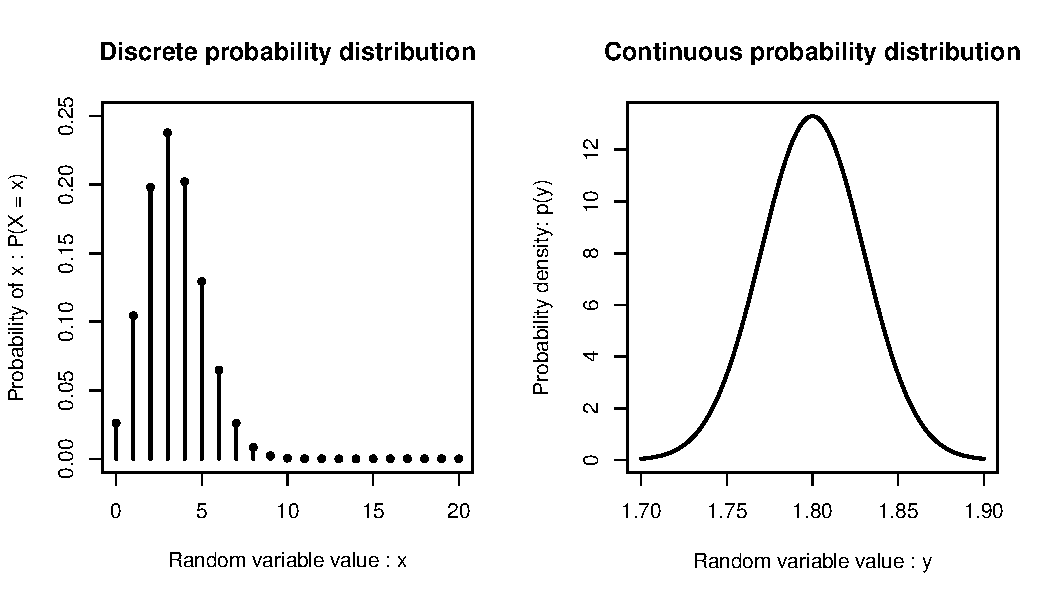
\includegraphics[width=\textwidth]{probability_distributions.pdf}
\caption{Left: Probability mass function. Right: Probability density function.}
\label{fig:example_pd}
\end{figure}
\begin{figure}
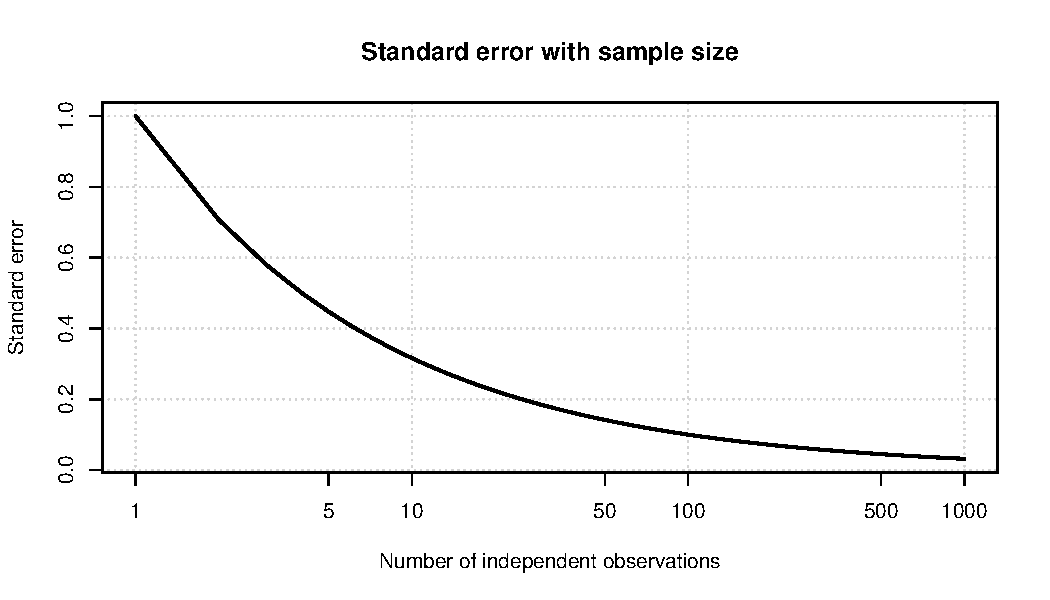
\includegraphics[width=\textwidth]{se_with_sample_size.pdf}
\caption{Convergence of sample mean to population mean.}
\label{fig:se_with_sample_size}
\end{figure}
\par


\subsection*{Tolerance Intervals}
DCA's most sophisticated statistical analysis is based on ISO 16269-6, \emph{Determination of statistical tolerance intervals}. This standard outlines how to construct tolerance intervals under either no assumptions about the random variable's distribution, or the assumption that the random variable has a normal distribution. A tolerance interval is a range of values that contain a particular fraction of the population to a given confidence level. A confidence level is the long-run proportion of intervals constructed that contain at least this proportion of the population. Consequently, tolerance intervals allow us to make statements about the performance of a population.
\par
We seek $k$ such that $\bar{x} + ks$ is greater than at least a proportion $p$ of the population with probability $1 - \alpha$. Let $\mu + u_p \sigma$ be greater than exactly a fraction $p$ of the population. Therefore:
\[
	P(\bar{x} + ks \geq \mu + u_p \sigma) = 1 - \alpha
\]
After some algebraic wrangling, it's possible to find:
\[
	P\Big(\frac{\sqrt{n}(\sigma u_p - \bar{x} + \mu)}{s} \leq \sqrt{n}k\Big) = 1 - \alpha
\]
The term on the l.h.s. of the inequality has a t-distribution with $n - 1$ degrees of freedom and location $\sqrt{n}u_p$. This means that 
\[
	\sqrt{n}k = t_{1 - \alpha}(\sqrt{n}u_p, n - 1)
\]
where $t_{1 - \alpha}(...)$ is the value corresponding to the $1 - \alpha$ percentile of the t-distribution with $n - 1$ degrees of freedom centered at $\sqrt{n}u_p$. The interval containing at least $p$ of the population with probability $1 - \alpha$ is therefore:
\[
	\Big(-\infty, \bar{x} + \frac{t_{1 - \alpha}(\sqrt{n}u_p, n - 1)\cdot s}{\sqrt{n}}\Big]
\]
This interval contains at least a fraction $p$ of the population with probability $1 - \alpha$. Example tolerance intervals are shown in Figure \ref{fig:tolerance_intervals}.
\begin{figure}
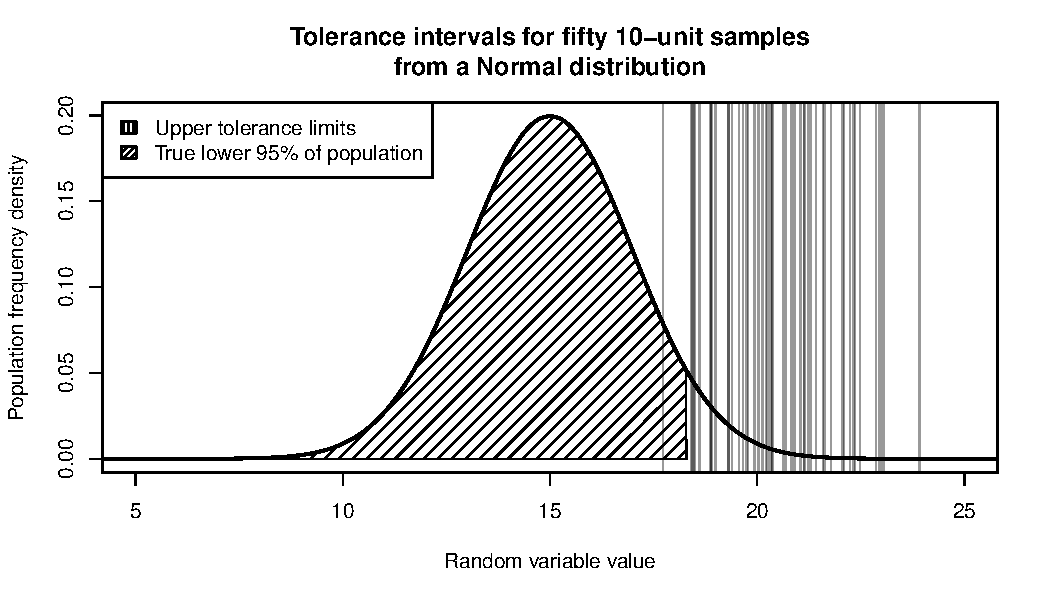
\includegraphics[width=\textwidth]{tolerance_intervals.pdf}
\caption{Example tolerance limits for a confidence level of 0.95. Each vertical line corresponds to a 95\% tolerance limit constructed for a simulated 10-unit sample.}
\label{fig:tolerance_intervals}
\end{figure}
At present, DCA do not test the assumption of Normality (check this).
% Questions:
%	> What is a t-distribution?
% 	> Do DCA test the normality assumption?
%	> 
\par
% Confidence intervals
Another tool that DCA's engineers occasionally use is confidence intervals. A confidence interval contains the value of a population parameter a proportion 1 - $\alpha$ of the cases in a long series of repeated random samples under identical conditions. They're useful when we want to quantify the uncertainty on our estimate of a population parameter such as the mean or variance. Again, these are applied in a presciptive manner, and the underlying assumptions are rarely checked. Rather than give a derivation of them here, they're suspended until Section X where they're shown in the context of Bayesian inference.
\subsection*{t-tests}
% Two-sample t-tests
THE FOLLOWING PLAGIARIZES MONTGOMERY AND SHALL BE CHANGED
Occasionally an analysis of a comparative test will contain a two-sample t-test. This assumes that the variances of the two groups tested is the same (i.e. the treatment may only affect the group mean, not its variance), and that the samples are randomly drawn from the same Normal distribution. The $p$-value obtained corresponds to the probability of observing the difference in sample means assuming that the two samples were drawn from the same Normal distribution. The implication of a small $p$-value is that assuming the two samples were drawn from the same Normal distribution is unreasonable. The two-sample t-test statistic is
\[
	t_0 = \frac{\bar{y}_1 - \bar{y}_2}{s_p^2 \cdot \sqrt{\frac{1}{n_1} + \frac{1}{n_2}}}
\]
Where $s_p^2$ is an estimate of the the two group's common variance $\sigma^2$:
\[
	s_p^2 = \frac{(n_1	 - 1)\cdot s_1^2 + (n_2 - 1)\cdot s_2^2}{n_1 + n_2 - 2}	
\]
If $t_0$ were greater than the value of t corresponding to the $\alpha/2$ percentage point of the t distribution with $n_1 + n_2 - 2$ degrees of freedom, we would reject $H_0$ and conclude that the means of the two groups differ.
\par
If we are sampling from independent Normal distributions, the the distribution of $\bar{y}_1 - \bar{y}_2$ is $N(\mu_1 - \mu_2, \sigma^2(1/n_1 + 1/n_2))$. Thus if the two distributions shared the same mean, then
\[
	Z_0 = \frac{\bar{y}_1 - \bar{y}_2}{\sigma\sqrt{\frac{1}{n_1} + \frac{1}{n_2}}}
\]
would be a $N(0, 1)$ r.v. However, because $\sigma$ is unknown, we must instead replace it with an estimate of the population standard deviation $s_p$, resulting in an r.v. that has a t-distribution.
\newpage
\subsection*{Monte Carlo estimation}
Monte Carlo simulation approximates a quantity by simulating the random process generating it . It has previously been applied within DCA to understand worst-case tolerances in products. The use case was somewhat similar to the following: the 95th percentile of some analytically inconvenient combination of distributions, each corresponding to a part dimension, was needed. Take $Y \sim \text{Binom}(n = 10, p = X)$ as an example, where $X \sim \text{Beta}(a = 7, b = 3)$\footnote{The beta distribution is a continuous and generates a number between $0$ and $1$, which makes it useful in modelling the distribution of a probability.}. Rather than attempt to derive the distribution of this dimension's value directly, tens of thousands of values of $y$ were first generated according to $Y$'s distribution using a computer. Each of these values were then used to generate a value of $x$ from $\text{Binom}(n = 10, p = y)$. The resulting frequencies of the $x$ values then represented the dimension's distribution. It was then possible to calculate the mean by averaging over all the $x$ values obtained. A diagram of this process is shown in Figure \ref{fig:monte_carlo}.
\begin{figure}[b!]
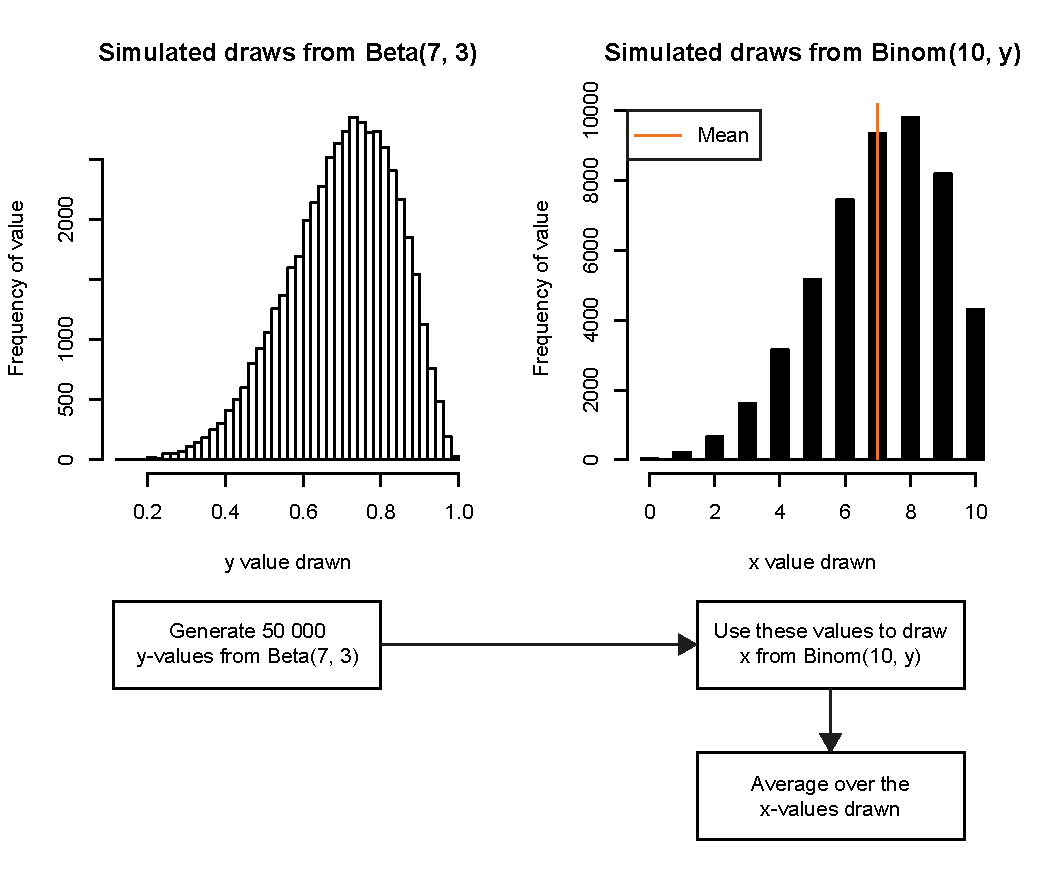
\includegraphics[width=0.8\textwidth]{monte_carlo_simulation.pdf}
\label{fig:monte_carlo}
\caption{Process diagram for a Monte Carlo simulation.}
\end{figure}


\newpage
\section{Visualizing Experimental Data}
DCA's reports and client presentations frequently contain plots of the data collected from an experiment. These plots are almost exclusively line charts or bar charts, with scatter plots also seeing occasional use. These figures are created using either Microsoft Excel or Matlab.
\par
The line chart in DCA is ubiquitous because it is directly plottable from the raw data provided by their axial and torsional testing machines. Typically a visual summary of a test consists of an overlay of many unit's results in a manner similar to Figure \ref{fig:line_plots}. 
\begin{itemize}
\item[+] Allows an entire test to be viewed simultaneously, providing a high-level summary of the results
\item[+] Is easily relatable to physical observations during a test
\item[+] Its meaning can be understood without explanation - it is a universally familiar chart
\item[-] Obscures the behaviour of individual units
\item[-] Encourages focus on extremes of group ranges, rather than the distribution of each group's performance
\item[-] Obfuscates data artifacts that aren't related to location or dispersion (such as harmonic content)
\item[-] May provide irrelevant information - it's often the case that only the peak or average values are of interest.
\end{itemize}
\begin{figure}
	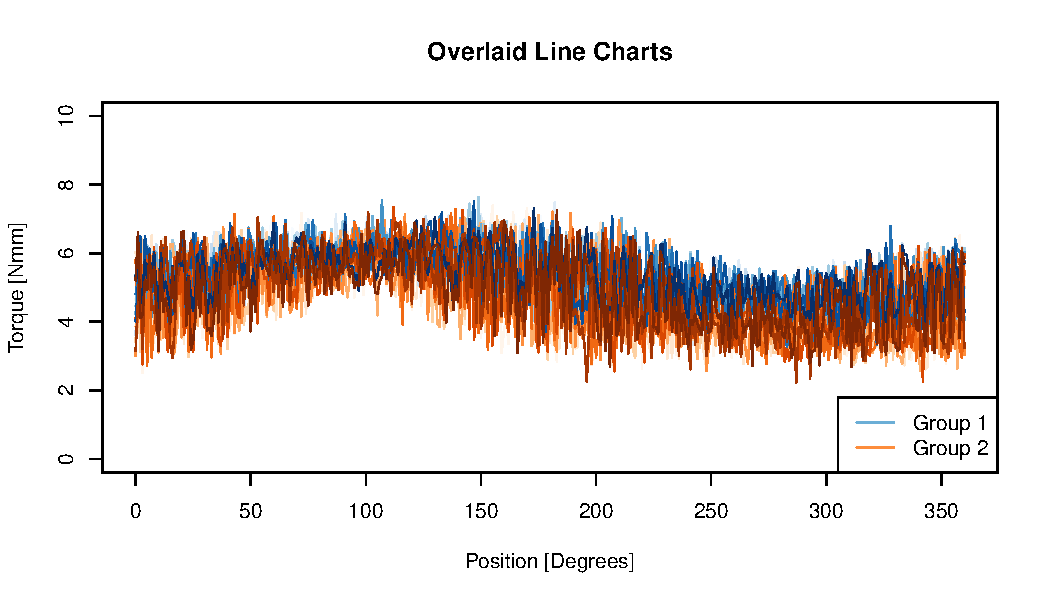
\includegraphics[width=\textwidth]{overlaid_line_charts.pdf}
	\label{line_plots}
	\caption{Sample summary line chart from a DCA test report.}
\end{figure}
The tolerance intervals in the preceding section are, by protocol, plotted according to the graph in Figure \ref{fig:tolerance_intervals_plot}. 
\begin{itemize}
\item[+] Something nice
\end{itemize}
\begin{figure}
	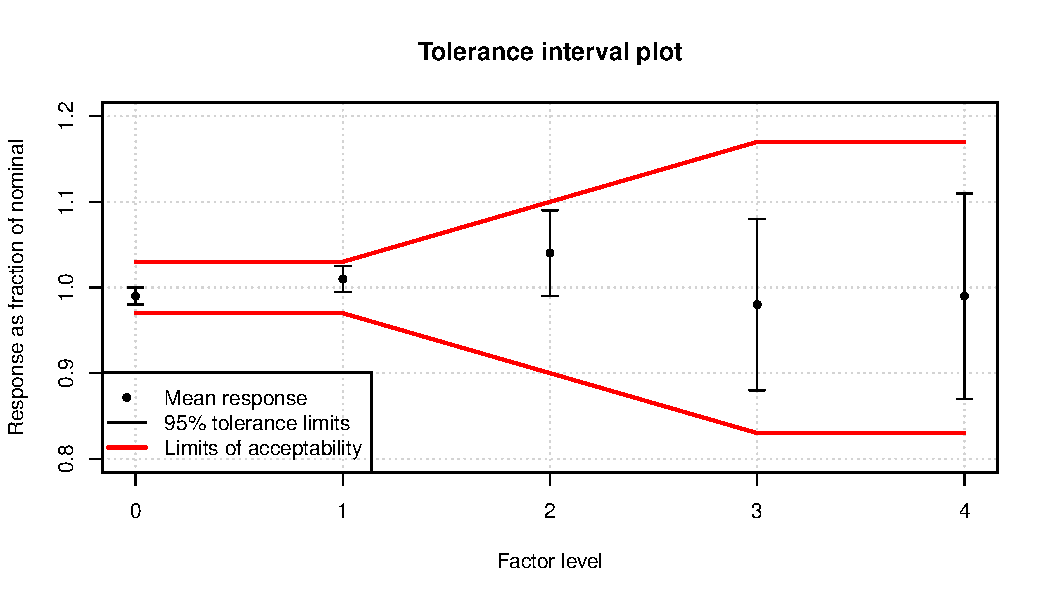
\includegraphics[width=\textwidth]{tolerance_intervals_plot.pdf}
	\label{tolerance_intervals_plot}
	\caption{Tolerance interval plot.}
\end{figure}

\section{Other Activities}

%%  SUGGESTED METHODS %%
\chapter{Suggested Methods}\label{suggested_methods}
\section{Experiment design}
\subsection*{Experimental pre-planning}
\subsection*{Fractional factorial designs}
\subsection*{Taguchi designs}

\section{Analysis}
\subsection*{Regression Models}
Regression models are a flexible tool that allow us to
\begin{itemize}
\item Estimate the effects of discrete and continuous factors on a unit's response - even if they interact or have a nonlinear influence.
\item Identify differences between units that aren't immediately apparent from raw data
\item Measure how well our understanding of a product lines up with its reality
\end{itemize}
\subsection*{Bayesian Inference}
\subsection*{Markov Chain Simulation}
\subsection*{Decision Trees}

%%
\section{Presentation \& Visualization}
\subsection{The Psychology of a Plot}
\subsection{Scatter plots}
\subsection{Histograms}
\subsection{Box plots}
\subsection{Separation Plots}
http://mdwardlab.com/sites/default/files/GreenhillWardSacks.pdf

%%
\section{Software}
\begin{itemize}
\item Excel
\item Matlab
\item R
\item Python
\item Minitab
\end{itemize}

\newpage


%% CONCLUSIONS AND RECOMMENDATIONS %%
\chapter{Conclusions \& Recommendations}

\newpage
\appendix
\chapter{}
Probability allows us to analyze a system without requiring complete mechanical knowledge of it. `'Randomness'' refers to sources of variation that aren't measured. You may have heard of probabilities as representing `'Degrees of belief''. To understand what a belief is, consider this example. We machine a coin that we check is a symmetric disk of homogeneous density. I flip the coin ten times, and it comes up heads every single time. You might be surprised by this, and accuse me of flipping it in a controlled way. I then ask you how I can flip it in a way that is fair. What is your response?
\par
If you say that it should come heads as many times as tails, then the experiment is no longer random, as we know what the outcome will be. You may gesticulate and say ``You need to flip it \emph{randomly}''. I would press you to tell me what this means - I require a mechanism to decide how to flip the coin, and physical mechanisms are deterministic.
\par
The probability of an outcome can only be evaluated to a set of assumptions you make about the mechanism generating those outcomes. You had a preconceived notion that the way I flipped the coin would favor neither heads nor tails, and therefore saw ten heads as supremely improbable.
\newpage
We can see this by recognizing that the sum of independent observation's variances is equal to the variance of the variance of the sum of the observations:
\begin{align}
 \text{Var}\sum_{i = 1}^n X_i &= \sum_{i = 1}^n \text{Var}X_i\\
	\text{Var}n\bar{X} &= n\text{Var}X \\
	\implies \sqrt{\text{Var}\bar{X}} &= \frac{\sigma}{\sqrt{n}}
\end{align}

% Ronald Fisher, The Design of Experiments
% Attacking the interpretation or data collection method
% `an experimenter... wishes to safeguard his results, ... from ignroant criticism by different sorts of superior persons'
% Criticizes Bayes' theorem: ` Advocates of inverse probability seem forced to regard mathematical probability not as an
%					objective quantity measured by observable frequencies, but as measureent merely
%					psychological tendencies'
% `Experimental observations are only experience planned in advance, and designed to form a secure basis of new knowledge'
% Refs: 	- An essay towards solving a problem in the doctrine of chances, T. Bayes (1763)

% R. Mead, Design of Experiments
% Introduction
% ---------------
% - Degrees of freedom - count of the number of independent comparisons that can be made
% - The total information in an experiment involving N experiental units may be represented by the total variation based on N -1 df
%		> Variation is divided into three components:
%			- Treatment component T, sum of df corresponding to the questions to be asked
%			- Blocking component B, representing all environment effects that are to be included in the fitted model.
%			  (b - 1)df for b blocks.
%			-  Error component E, used to estimate the error's variance (i.e. estimate the standard errors)
%	The resource equation:	T + B + E = N - 1
%	To obtain a good estimate of error, need at least 10 df (preferably 15)
%	- Calculable by examining the 5% point of the t-distribution, and using enough df that increasing the error df
%	  makes little difference to the significance value.
%
% One final comment on this question of efficient use of resources. It is, of course, possible
% to keep the value of E in the region of 10–20 by doing several small experiments, rather than
% one rather larger experiment in which the total number of experimental units is much less
% than the sum of the units in the separate small experiments. This is inefficient because of the
% need to estimate σ2 for each separate experiment. Experimenters should identify clearly the
% questions they wish the experiment to cover, and they should also consider carefully if they
% are asking enough questions to use the experimental resources efficiently.

% Randomized complete block design: Essentially each group of ‘similar’ units
%					        should include roughly equal numbers of units for each treatment. 
%					        This control is referred to as blocking.
%						- `Similar' units -> e.g. same spring orientation, batch numbers, cavity numbers
%					       Each block contains a single replicate of each of the treatments.
%					       Key idea is to make groups subject to similar sources of variation.
%					      A `block' is a group of similar units.
% Completely randomized design: Randomly allocate treatments to units.
%

% Analysis of variance
% - Provides a subdivision of the total variation between the exerimental units into separate components, each component
%	representing a different source of variation, so that the relative importance of the different sources can be assessed.
% - Gives and estimate of the underlying variation between units, providing a basis for inferences about the applied
%	treatments.
% The basic philosophy of analysis of variance is to assume that each unit has an inherent
% response, possibly related to the position of the unit within the experiment, which is modified
% by the effect of the particular treatment applied to the unit.
% Response in terms of components y_{ij} = \mu + b_i + t_j _ \epsilon_{ij}
% \mu is the average of the whole set of experimental units, b_i is the term representing the average deviation
% from \mu of the units in block i, t_j is the term representing the average deviation from the \mu of the units given treatment j,
% \epsilon_{ij}  represents the deviation of a particular unit from \mu + b_i.
% sum over t_j must equal zero, as must the sum over b_i.
% Assumptions: - Individual unit variation is not affected by treatment applied to the unit.
%		      - The effect of each treatment is additive - the chosen block does not affect the efficacy of the treatment.
% The analysis of variance of data from an experimental design is simply the division of the
% total variation between the n observations into sensibly distinguishable components, and the
% subsequent interpretation of the relative size of the components
% Applying this principle to the randomized block design, we get
% \[
%	total SS = block SS + treatment SS + error SS
% \]
% Standard error of the difference between treatments
% In addition, it is natural, when making comparisons, to concentrate on
% those comparisons which look larger, which will be between the treatments giving the more
% extreme results and which are then subject to a selection bias.n addition, it is natural, when making comparisons, to concentrate on
% those comparisons which look larger, which will be between the treatments giving the more
% extreme results and which are then subject to a selection bias.

% Multiple blocking and recording of nuisance variables
\end{document}